\documentclass[12pt, a4paper]{article}
\setlength{\parindent}{0cm}
\usepackage[margin=1in]{geometry}
\usepackage[english]{isodate}
\cleanlookdateon

\usepackage[hidelinks=true]{hyperref}
\usepackage{graphicx}
\usepackage{float}
\usepackage{listings}
\usepackage[usenames,dvipsnames]{color}    
\lstset{
  basicstyle = \small\ttfamily,
  backgroundcolor = \color{White},
  showstringspaces = false,
  frame = single,
  rulecolor = \color{Black},
  tabsize = 4,
  breaklines = true,
  breakatwhitespace = false,
  keywordstyle = \color{RoyalBlue},
  commentstyle = \color{YellowGreen},
  stringstyle = \color{ForestGreen}
}

\usepackage[style=apa]{biblatex}
\addbibresource{sample_ref.bib}

\title{Run Directory Automatically for a Research Project}
\author{Qichao Wang\thanks{I am a PhD student in Economics in the Department of Economics at The Hong Kong University of Science and Technology. Email: \href{mailto:qwangcq@connect.ust.hk}{qwangcq@connect.ust.hk}.}}
\date{\today}

\begin{document}

\maketitle

A research project involves a lot of steps. Generally, there are the following steps:
\begin{itemize}
	\item Data cleaning
	\item Data transformation
	\item Data analysis
	\item Literature review
	\item Paper writing
\end{itemize}
However, each step requires at least some manual work. Sometimes the data steps involve multiple statistical software. For example, a project in macroeconomics possibly involves processing raw data in Stata before further analysis in Matlab. When the number of software used increases, manual work can be laborious. To liberate researchers from manual work, automation at a higher degree is desirable.\\

I was illuminated by \textcite{gentzkow_code_2014} to adopt the complete automatic process for a research project as an additional step from a manual pipeline from data processing and plotting using Stata, R or Matlab to typesetting the research paper using \LaTeX. The Python programme is based on \textcite{hofman_github_2018}'s work with modifications.\\

The report is automatically generated down the line from the python script file \texttt{rundirectory.py}. I include the functions in another file \texttt{rundirectory\_function.py} with necessary pre-settings, including the directories to call the software in the Mac terminal. All the contents in the handbook are self-contained in the code files.\\

\section{Stata}

The automation can handle Stata files. The caveat is that the only plot format the terminal version of Stata supports is eps.\\

Currently, I optimise the compatibility of the Stata processing, so it works in both a Mac environment and a Windows environment.\\

I run the following Stata code.\footnote{I use the first data file from: \url{https://stats.oarc.ucla.edu/stata/examples/kirk/experimental-design-procedures-for-the-behavioral-sciences-third-edition-by-roger-e-kirk/} here for illustrative purposes.}\\

\lstinputlisting{sample_stata.do}

The function to run Stata code, \texttt{run\_stata}, is as follow.\\

\lstinputlisting[language=Python, linerange={23-44}]{rundirectory_function.py}

The output plot is as follows.\\

\begin{figure}[H]
	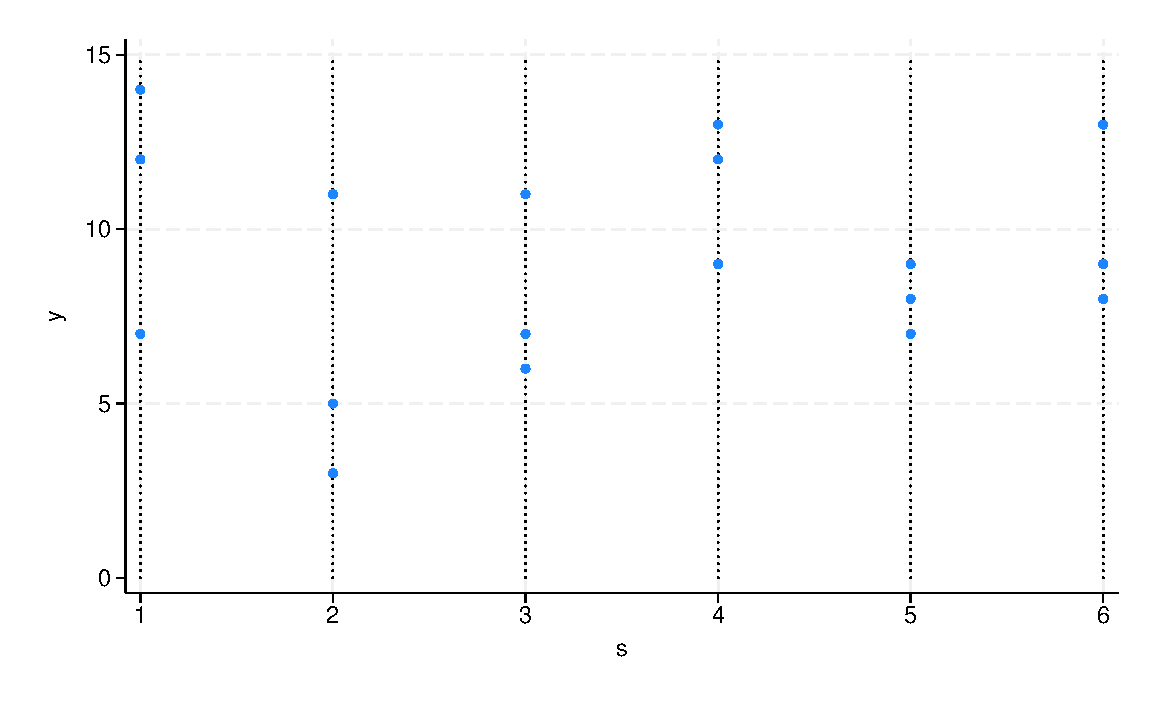
\includegraphics[width=.5\textwidth]{sample_stata_graph}
\end{figure}

\section{R}

The automation can handle R files. I have not yet found the solution to use the Mac terminal to open a project in RStudio, run an R script within the project, and then close the project. However, I can still run R scripts using all functions generated in the clean-and-install process of the project. Just load the library named after the project, and the functions are available. To use the processing on an RStudio project, add a line at the top of the R script to set the working directory as the root folder where the \texttt{.Rproj} file is located.\\

I run the following R code.\\

\lstinputlisting[language=R]{sample_r.R}

The function to run R code, \texttt{run\_python}, is as follow.\\

\lstinputlisting[language=Python, linerange={46-52}]{rundirectory_function.py}

The output plot is as follows.\\

\begin{figure}[H]
	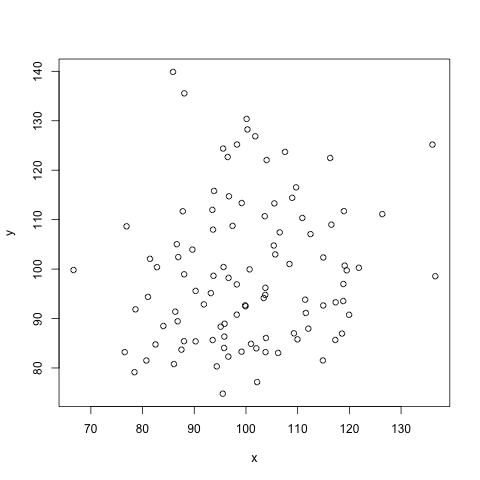
\includegraphics[width=.5\textwidth]{sample_r_graph.png}
\end{figure}

\section{Matlab}

The automation can handle Matlab files. Running scripts within a project environment is supported for Matlab processing. Nesting batch processing with parallel computing within a script substantially boosts efficiency. Dynare codes can also be nested within the script.\\

I run the following Matlab code.\\

\lstinputlisting[language=Matlab]{sample_matlab.m}

The function to run Matlab code, \texttt{run\_matlab}, is as follow.\\

\lstinputlisting[language=Python, linerange={54-60}]{rundirectory_function.py}

The output plot is as follows.\\

\begin{figure}[H]
	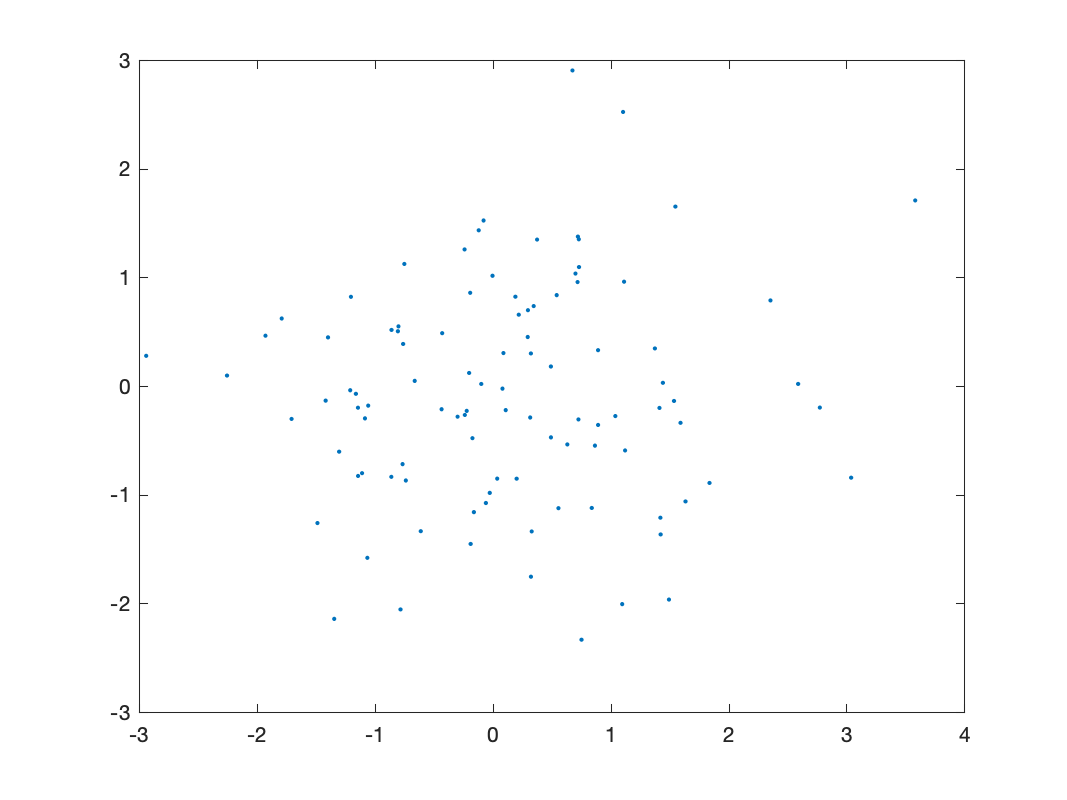
\includegraphics[width=.5\textwidth]{sample_matlab_graph.png}
\end{figure}

\section{Python}

The automation can handle Python files. Therefore, we can implement the automation process recursively.\\

I run the following Python code.\\

\lstinputlisting[language=Python]{sample_python.py}

The function to run Python code, \texttt{run\_python}, is as follow.\\

\lstinputlisting[language=Python, linerange={62-68}]{rundirectory_function.py}

The output plot is as follows.\\

\begin{figure}[H]
	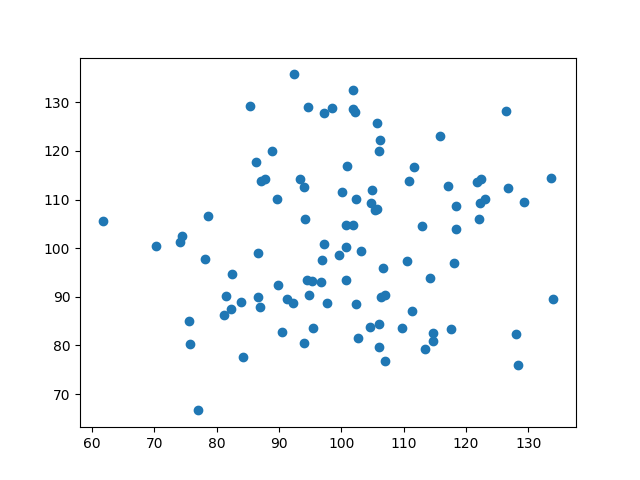
\includegraphics[width=.5\textwidth]{sample_python_graph.png}
\end{figure}

\section{LaTex}

Finally, everything is poured into the LaTeX for final processing towards the research report. The function to run LaTeX, \texttt{run\_latex}, is as follows.\\

\lstinputlisting[language=Python, linerange={70-84}]{rundirectory_function.py}

Note that the function has three arguments. The second specifies the number of typesettings after loading the BibTex. The default setting is two, when the processing typesets the pdf file twice after loading the references. The third, a logical variable, specifies whether external tools are needed for the Tex compiling. It should be enabled (set to \texttt{True}) when the compile needs to access files outside the folder of the Tex file.\\

\section{Automation}

To run the whole process, just open the Python script of \texttt{rundirectory.py} and run. It automatically includes functions and pre-settings from the function script.\\

To change the location of the software used, open \texttt{rundirectory\_function.py} and manually modify the section under ``locations of the software". We can extend the terminal processing to any statistical software that supports running at the terminal.\\

The main script, \texttt{rundirectory.py}, is as follows.\\

\lstinputlisting[language=Python]{rundirectory.py}

For Mac users, click the folder that contains the main script, then click ``Finder" $->$ ``Services" $->$ ``New Terminal at Folder". In the popped terminal, type:
\begin{verbatim}
	python3 rundirectory.py
\end{verbatim}
and return, and then the script starts to run automatically.\\

\nocite{*}
\printbibliography

\end{document}
